\documentclass{article}
\usepackage[a4paper, margin={1in, 1in}]{geometry}
\usepackage[utf8]{inputenc}
\usepackage{polski}
\usepackage{mathtools}
\usepackage{amsfonts}
\usepackage{amssymb}
\usepackage{amsmath}
\usepackage{multicol}
\usepackage{paralist}
\usepackage{tabto}
\usepackage{graphicx}
\usepackage{etoolbox}
\usepackage{changepage}
\usepackage{tasks}
\usepackage{pgfplots}
\usepackage{fancyhdr}

\DeclareMathOperator{\arctg}{arctg}
\DeclareMathOperator{\sh}{sh}
\DeclareMathOperator{\ch}{ch}
\DeclareMathOperator{\sgn}{sgn}

\let\arctan\relax
\DeclareMathOperator{\arctan}{arctg}
\let\tan\relax
\DeclareMathOperator{\tan}{tg}

% Dodatkowe deklaracje:

\usepackage{subcaption}

\usetikzlibrary{patterns}
\usetikzlibrary{intersections}
\usepgfplotslibrary{fillbetween}

\newcommand{\Because}{\quad\because\quad}
\newcommand{\case}[1]{\textrm{#1$^\circ$}}
\newcommand{\degree}{^{\circ}}
\newcommand{\diff}{\mathop{}\!\mathrm{d}}
\newcommand{\for}{\ \leftrightarrow\ }
\newcommand{\Integral}[4]{\int_{#1}^{#2} \! #3 \, \mathop{}\!\mathrm{d}#4}
\newcommand{\mathcolorbox}[2]{\colorbox{#1}{$\displaystyle #2$}}
\newcommand{\norm}[1]{\left\lVert#1\right\rVert}
\newcommand{\qed}{\textbf{\textit{QED}}}
\newcommand{\qef}{\textbf{\textit{QEF}}}
\newcommand{\task}[1]{\textit{#1}}
\newcommand{\xrowht}[2][0]{\addstackgap[.5\dimexpr#2\relax]{\vphantom{#1}}}
\newcommand{\partderiv}[2]{\frac{\partial #1}{\partial #2}}

\DeclareMathOperator{\?}{?}
\DeclareMathOperator{\dom}{dom}
\DeclareMathOperator{\im}{im}
\DeclareMathOperator{\lin}{lin}
\DeclareMathOperator{\N}{\mathbb{N}}
\DeclareMathOperator{\R}{\mathbb{R}}
\DeclareMathOperator{\Z}{\mathbb{Z}}

\let\oldepsilon\epsilon \renewcommand{\epsilon}{\varepsilon}

% Koniec dodatkowych deklaracji

\pagestyle{fancy}

\lhead{Analiza Matematyczna 2; 2020/2021}
% Tutaj proszę uzupełnić imię i nazwisko
\rhead{Jakub Łukasiewicz}

\begin{document}
\section*{Zadanie 1c}

Obliczyć $\displaystyle \iiint_U x^2 + y^2 \ \diff{x}\diff{y}\diff{z}$, gdzie
$U: x^2 + y^2  \le 4, 1-x \le z \le 2-x$

\subsection*{Rozwiązanie}

Rzut $D_{xy}$ obszaru $U$ na płaszczyznę $xOy$ :
\begin{figure}[h!]
   \centering
   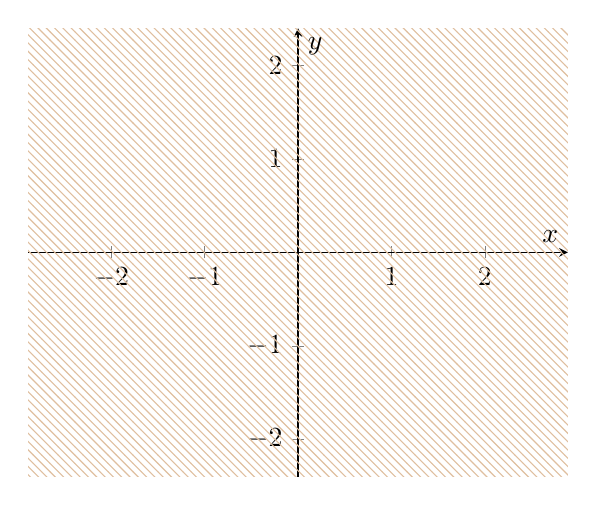
\begin{tikzpicture}
      \begin{axis}[
            xmin=-2,xmax=2,
            ymin=-2,ymax=2,
            axis x line=middle,
            axis y line=middle,
            axis equal,
            enlargelimits,
            xlabel={$x$},
            ylabel={$y$},
         ]
         \draw [blue, pattern=north west lines, pattern color=brown!50] (axis cs: 0, 0) circle [radius=200];
      \end{axis}
   \end{tikzpicture}
\end{figure}

\noindent Obszar $U$ jest ograniczony z dołu powierzchnią o równaniu
$z = D(x,y) = 1-x \for (x,y) \in D_{xy}$, \\
a z góry o równaniu $z = G(x,y) = 2-x \for (x,y) \in D_{xy}$.

\begin{equation*}
   x^2 + y^2 \le 4 \implies -\sqrt{4-x^2} \le y \le \sqrt{4-x^2}
\end{equation*}

\begin{equation*}
   \Integral{1-x}{2-x}{x^2 + y^2}{z} = (x^2 + y^2)[z]_{x-1}^{2-x} = (x^2+y^2)(2-x-x+1) = (3-2x)(x^2+y^2) = f(x,y)
\end{equation*}

\begin{equation*}
   \Integral{0}{\sqrt{4-x^2}}{f(x,y)}{y} =
   (3-2x)\left[x^2 y + \frac{y^3}{3} \right]_0^{\sqrt{4-x^2}} =
   (3-2x)\left(x^2\sqrt{4-x^2} + \frac{\sqrt{4-x^2}^3}{3} \right) = g(x)
\end{equation*}

\begin{equation*}
   \Integral{-\sqrt{4-x^2}}{0}{f(x,y)}{y} =
   (3-2x)\left[x^2 y + \frac{y^3}{3} \right]_{-\sqrt{4-x^2}}^0 =
   (3-2x)\left(-x^2\sqrt{4-x^2} - \frac{\sqrt{4-x^2}^3}{3} \right) = -g(x)
\end{equation*}

\begin{equation*}
   \ldots\ ?
\end{equation*}

\clearpage
\section*{Zadanie 3d}

Wprowadzając współrzędne sferyczne obliczyć
$\displaystyle \iiint_U x^2 \ \diff{x}\diff{y}\diff{z} $,
gdzie $U: x^2 + y^2 + z^2 \le 4x$

\subsection*{Rozwiązanie}

\begin{gather*}
   x^2 + y^2 + z^2 \le 4x \\
   x^2 - 4x + 4 - 4 + y^2 + z^2 \le 0 \\
   (x^2 - 2)^2 + y^2 + z^2 \le 4
\end{gather*}

Obszar $U$ to kula o środku $(2,0,0)$ i promieniu $2$.
Zatem $0 \le \varphi \le 2\pi$, $-\frac{\pi}{2} \le \phi \le \frac{\pi}{2}$ oraz $2 \le \varrho \le 4$.

Dokonujemy zmiany na zmienne sferyczne:

\begin{equation*}
   \begin{aligned}
      \iiint_U x^2 \ \diff{x}\diff{y}\diff{z} &=
      \Integral{0}{2\pi}{}{\varphi}
      \Integral{-\frac{\pi}{2}}{\frac{\pi}{2}}{}{\phi}
      \Integral{2}{4}{\varphi^2}{\varrho}
      =
      \Integral{0}{2\pi}{}{\varphi}
      \Integral{-\frac{\pi}{2}}{\frac{\pi}{2}}{2\varphi^2}{\phi}
      =\\ &=
      \Integral{0}{2\pi}{2\pi \varphi^2}{\varphi}
      =
      2\pi \left[\frac{x^3}{3}\right]_0^{2\pi}
      =
      2\pi \frac{8\pi^3}{3} = \frac{16\pi^4}{3}
   \end{aligned}
\end{equation*}

\subsection*{Odpowiedź}
\begin{equation*}
      \iiint_U x^2 \ \diff{x}\diff{y}\diff{z} = \frac{16\pi^4}{3}
\end{equation*}

\clearpage
\section*{Zadanie 1a}

Obliczyć $\displaystyle \iiint_U e^{x+y+z} \ \diff{x}\diff{y}\diff{z}$, gdzie
$U: x \le 0, \ -x \le y \le 1, \ 0 \le z \le -x$

\subsection*{Rozwiązanie}

Rzut $D_{xy}$ obszaru $U$ na płaszczyznę $xOy$ :

\begin{figure}[ht!]
   \centering
   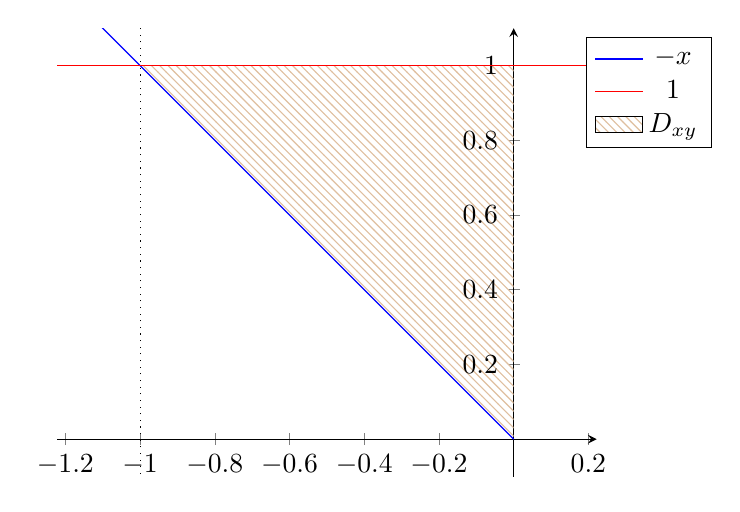
\begin{tikzpicture}
      \begin{axis}[
            xmin=-1,xmax=0,
            ymin=0,ymax=1,
            axis lines=middle,
            axis equal,
            enlargelimits,
            domain=-2:0,
            samples=3,
            legend style={anchor=north west}]
         ]
         \addplot[name path=F, blue] {-x};
         \addplot[name path=G, red]  [domain=-2:2]{1};

         \addplot[pattern=north west lines, pattern color=brown!50]fill between[of=F and G,  soft clip={domain=-1:0}];

         \addplot +[mark=none, dotted] coordinates {(-1, -1) (-1, 2)};

         \legend{$-x$, $1$, $D_{xy}$}
      \end{axis}
   \end{tikzpicture}
\end{figure}

\noindent Obszar $U$ jest ograniczony z dołu powierzchnią o równaniu $z = D(x,y) \equiv 0$,
a z góry o równaniu $z = G(x,y) = -x \for (x,y) \in D_{xy}$.

\vspace{1em} Zamieniając całkę potrójną na iterowane:

\begin{equation*}
   \begin{aligned}
      \iiint_U e^{x+y+z} \ \diff{x}\diff{y}\diff{z}
      &=
      \Integral{-1}{0}{}{x}
      \Integral{-x}{1}{}{y}
      \Integral{0}{-x}{e^{x+y+z}}{z}
      =
      \Integral{-1}{0}{}{x}
      \Integral{-x}{1}{e^{x+y} \big[e^z\big]_{z=0}^{z=-x}}{y}
      =\\ &=
      \Integral{-1}{0}{}{x}
      \Integral{-x}{1}{e^{x+y} (e^{-x} - 1)}{y}
      =
      \Integral{-1}{0}{}{x}
      \Integral{-x}{1}{e^x (e^{-x} - 1) e^y}{y}
      =\\ &=
      \Integral{-1}{0}{(1 - e^x) \big[e^y\big]_{y=-x}^{y=1}}{x}
      =
      \Integral{-1}{0}{(1 - e^x) (e - e^{-x})}{x}
      =\\ &=
      \Integral{-1}{0}{(e - e\cdot e^x - e^{-x} + 1)}{x}
      =  3 - e
   \end{aligned}
\end{equation*}

\subsection*{Odpowiedź}

\begin{equation*}
   \iiint_U e^{x+y+z} \ \diff{x}\diff{y}\diff{z} = 3 - e
\end{equation*}

\end{document}
